
\chapter{引言}
\label{chapter:intro}

\section{研究背景}
有赖于计算机互联网技术,计算机存储和计算技术的快速发展,计算机应用已经深入地影响并改变了人类的生活。本人非常庆幸能够出生在20世纪末,赶上了一个新的计算机技术浪潮,并身处在这个环境中。

计算机技术的广泛应用所带来的互联网信息爆炸,以及大数据处理技术发展已经是老生常谈的话题了。然而它们给人类带来的机遇和挑战从来不会中断和消逝,计算机技术的发展的动力正是来源于这种源源不断的冲击。

IDC预测,到2020年第三代信息技术平台的市场规模将达到5.3万亿美元,到2020年,IT产业$90\%$的增长将由第三代信息技术平台驱动。
\subsection{流式数据}

美国图灵奖得主,诺贝尔经济学奖获得者赫伯特$\cdot$西蒙(Herbert A.Simon, $1916\sim2001$)曾说过:“在信息时代,最稀缺的资源不在是信息本身,而是对信息的处理能力。”

什么是大数据,迄今没有公认的定义。相较于传统的数据,人们将大数据的特征总结为5个V,即体量大(volume)、速度快(velocity)、模态多(variety)、难辨识(veracity)和价值大密度低(value)\cite{cxq2014Survey}。但大数据的主要难点并不在于体量大,真正难以应付的问题来自于其他几种特性。在这种环境下,人们往往遇到的是非结构化,海量实时的文本、视频、语音数据。这些数据常常意味着更大的技术挑战和更复杂的计算,以及更长的计算时间。而在商业应用中,数据处理的时间和质量往往意味着利益。

在许多应用场景中,数据是一个无穷的序列,并且数据的来源各异,格式复杂多样,数据可能带有一些时序,但是有无法保证数据是按照时间顺序排列处理。通常这类数据被称为流式数据。在不同场景下流式数据呈现出不同的特征,但是他们仍然具有鲜明的共性:

(1) 无限性。在流式场景下,数据以元组为单位,以连续的数据流的形式持续地到达计算系统。

(2) 无序性。虽然每个元组会按照某种时间顺序产生,但是,数据并不是严格按照时间次序到达。

(3) 突发性。数据的流速大小、元组特性数量和数据格式无法被提前预知。

(4) 易失性。在流式场景下,累加的数据量非常巨大。通常来说,数据通过简单的计算之后便会被丢弃,而不会别存储。

(5) 实时性。流式数据不仅是实时产生的,而且要求实时的返回计算结果。短时间内无法返回结果的数据,将会很大的影响系统的性能。

许多分布式计算系统都可以实时或接近实时地处理流式数据。常见的处理系统包括Storm, Spark Streaming和Samza。
Storm是一个实时的数据计算系统,使用过程中会先设计好一个用于实时计算的拓扑结构。Storm的数据流单位是元组,每个元组都是一个不可变的数组。
Spark Streaming是核心Spark API的一个扩展。它并不会像Storm那样一次一个地处理数据流。而是在处理之前按照时间间隔预先将其切分为一批次一批次的批处理作业。数据流被抽象为DStream数据结构,每个微处理批次得到一个RDD。
Samza处理数据流是,会分别按次处理每条收到的消息,但是Samza的刘单位既不是元组也不是DStream,而是一条条消息。

\subsection{流式数据场景}
比较典型的流式计算场景包括金融银行业应用、互联网应用和物联网应用\cite{sun2013bdsc}。
在互联网应用场景中,用户通常通过实时发布和分享产生各类数据,这其中最为典型的包括twitter,微博等社交软件的使用。
据统计,互联网上的数据有$75\%$来自于个人用户,主要有文本,图片、音频和视频等数据形式。


随着互联网的快速发展和壮大,网络已经融入到我们生活的方方面面,
用户可以方便的使用互联网进行检索、购物、娱乐、交流等活动。
根据CNNIC发布的《第39次中国互联网发展状况统计报告》显示,截至2016年12月,
我国网民规模达7.31亿,相当于欧洲人口总量,互联网普及率达到$53.2\%$\cite{website:cnnic-39}。

\begin{figure}[htb]\centering
  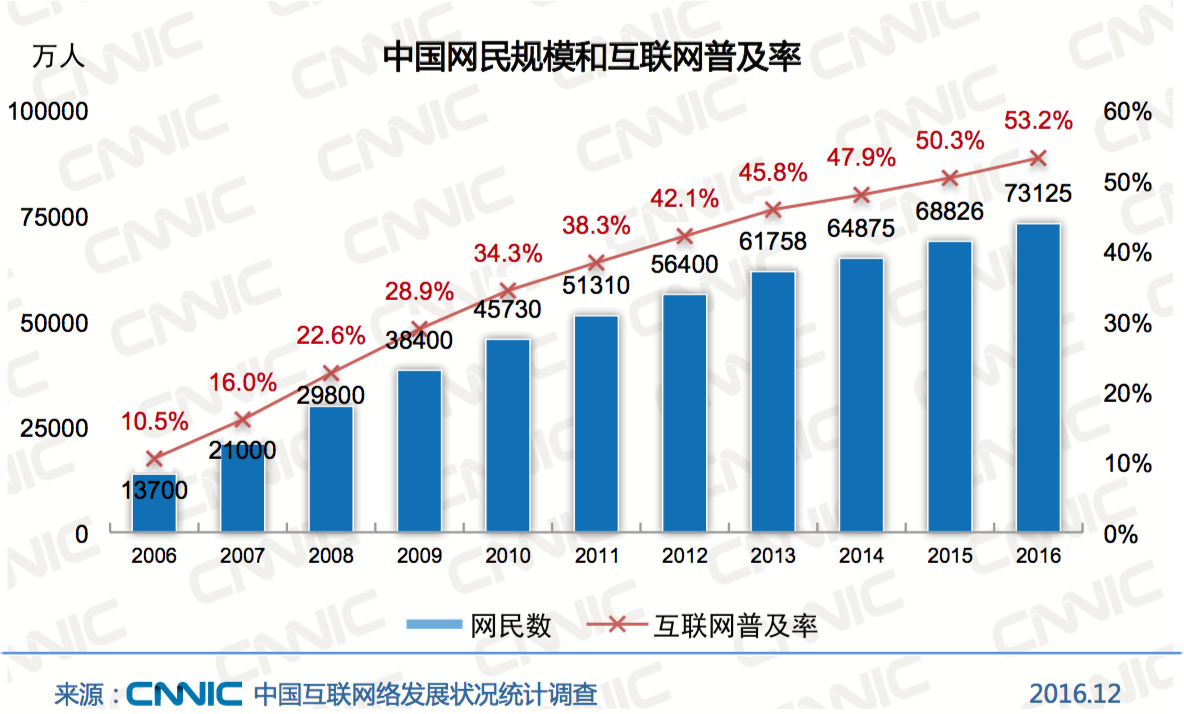
\includegraphics[width=0.7\linewidth]{cnnic-39-netuser}
\caption{中国网民规模和互联网普及率}
\label{fig:cnnic-39-netuser}       % Give a unique label
\end{figure}

社交网络以其快速灵活的方式己经逐渐改变人们交流的方式,用户可以在社交网络上进行沟通、分享、娱乐等活动。
以微博为例,微博是一个拥有庞大的用户基础,月活跃用户数(MAU)达到3亿的社交应用。
相对于传统的社交媒体,微博的时效性更强,影响范围更大,活跃度更高。微博月阅读量超百亿的领域达到了18个。
泛娱乐领域是微博活跃的主力场所;此外,在财经、教育、动漫等领域,微博同样发展迅速,颇受用户关注。
由于微博的流行与普及,微博信息数量呈爆炸式的增长,针对微博数据的处理和应用体现出典型的流式数据处理特征。

\subsection{流式数据与机器学习}
互联网的发展不仅推动了产业革命,同时也促进了机器学习人工智能的发展。人们常说在互联网时代,互联网是基础设施,数据就像原油。
那么机器学习就充当着高效提炼石油的技术。大数据与机器学习人工智能的结合,数据创造价值的关键。
每年Google,Facebook, Microsoft,百度,阿里等等国内外巨头公司都会在这些技术上有巨大的投入。
iResearch预测,2020年,中国人工智能市场将从2015年的12 亿人民币增长至 91 亿人民币。
2015 年,约 14 亿资本(年增长率 $76\%$)流入了中国的人工智能市场。机器学习人工智能俨然已经成为了各大公司的必争之地。

如上面所提及的,社交网络数据带有典型的流式数据特征,类似的场景还有许多。然而在流式数据环境下,传统的批量机器学习方法不再适用。
传统批量机器学习方法在流式数据环境下遇到了如下几个限制:

(1) 有限性

批量机器学习算法为了优化目标函数,会存储有限的训练集。流式数据具有无限性,数据持续的产生和输入,而无法完全存储在内存中。

(2) 迭代性

批量机器学习算法一般需要多轮迭代。在流式场景下,数据具有易失性和实时性,因此对算法的时间效率要求很高。通常数据仅经过简单的计算之后便会被丢弃。
因而,迭代性无法得到保障。

(3) 稳定性

批量机器学习算法都是基于独立同分布假设的。流式环境下,数据的分布可能随时间的推移而变动。因而,独立同分布假设无法得到保证。

(4) 静态性

批量机器学习算法训练得到的模型是静态的。在流式环境下,模型通常需要被实时地更新。使用静态的模型,则模型需要被频繁的替换,从而会造成应用系统的不稳定。

针对这些问题研究者也提出了一些在流式数据上的机器学习算法。
这些算法通常考虑了模型在时间上的延续性,消耗较少的内存,对数据变动具有感知能力。

P.Domingos和G.Hulten\cite{Domingos01catchingup}很好地总结了高效挖掘连续,高速,无尽的数据流学习系统的特性:

(1) 对每个数据样本只需要很少的运算时间

(2) 使用内存大小固定,与处理的样本数据总量无关

(3) 在构建模型的过程中,所有训练数据只会被计算一遍或少数几遍

(4) 随时产生独立于样本顺序的模型

(5) 具有概念迁移能力

\subsection{主题模型}
主题模型(Topic Model)在机器学习和文本挖掘领域是用来发现一系列文档中潜在语义主题的一种常用统计模型。
主题模型具有表征文本的作用,在社交网络文本数据中具有广泛的应用,对互联网的技术的影响是巨大的。
许多公司都有自己大规模主题模型实现,主要用于广告、推荐和检索等系统中。

现有的比较具有代表性的对规模主题模型实现包括LightLDA\cite{yuan2015lightlda}和PLDA+\cite{Liu:2011:PPL:1961189.1961198},以及Peacock\cite{Peacock}。
这些算法实现快速高效,扩展性也很好。但是,这些算法实现无一不是为静态数据集设计的。而在流式数据环境下,算法将面临的是开放无限的数据集,持续增长的词表以及不断演变的数据分布。
显然,现有的算法无法克服上面的问题挑战。

本文的主要工作是在流式数据环境下实现在线的主题模型。

\section{研究意义}

主题模型提供了一种从大规模数据中发现文本潜在语义只是的方法,并且将字词、文档映射到高维的语义空间上。
这种计算对很多语义相关的应用很有帮助,比如信息检索、推荐系统等等。
在社交网络文本分类和文本语义挖掘的应用中,主题模型同样具有重要的作用。

当谈及流式机器学习的时候,人们往往需要:
(1) 模型具有时效性。比如天气,如果前两天的天气都是晴天40度,那么第三天下雪的可能性就几乎不可能了。
(2) 模型被经常更新。这需要模型对流数据的烟花和结构具有感知。

本文主要工作是研究流式环境下大规模参数模型的学习和实现。考虑到流式环境下模型的时效性,和经常被更新,批量机器学习算法不再适用。
解决这个方法的途径通常是增量学习和在线学习。区别于批量学习,增量学习和在线学习每次只会适用一小批次的数据(而不是整个数据集),并且数据的信息也可能随着时间的变化而产生变化。
这类方法能够渐进地学习到知识更新演化,并且能修正和加强已有的知识,使得更新后的只是能够适应新的数据,而不必重新对全部数据进行迭代学习。
增量学习和在线学习降低了算法对时间和控件的要求,更适应与流式数据环境。

但是在流式数据环境下主题模型的实现仍然存在挑战:

(1) 流式数据的特点带来的挑战

在流式数据环境下,数据带有实时性和无限性。而经典的主题模型实在静态数据上采用批量学习算法更新模型的,因而无法支持算法的实时性和在线更新。
除此之外,无限的数据意味着动态增长的词表,而词表的大小决定了主题模型的参数个数。根据词汇的幂律分布法则,我们知道随着时间的推移,不断会有新词出现,而绝大多数词汇确实低频词。

(2) 大规模的数据带来的挑战

在社交网络场景下,动辄上亿的数据使得单机机器学习算法无法快速实时地更新模型和作出即使响应。

(3) 主题模型拥有大规模的参数矩阵

主题模型的参数规模,数据词表大小以及主题的维度大小有关。主题模型的参数规模常常超出了一台服务所能存储的容量。不仅如此,在分布式环境下,更多的参数往往意味着更长的网络延迟。

面对如此复杂的算法和应用场景,对主题模型的研究不仅具有现实意义,而且还具有一定的代表性。比如,大规模流式数据上的机器学习模型和大规模参数模型,不仅仅在主题模型这个算法中会出现,同样还会出现在一些其他机器学习算法的应用中。

\section{本文贡献}
为了解决分布式流式数据环境下,主题模型实现遇到的挑战。本文分析

(1) 提出了分布式流式主题模型

(2) 采用了高效的Metropolis-Hastings算法

(3) 提出了稠密和稀疏并存的分布式参数数据结构


\section{章节安排}
第二章
第三章 将主要介绍流式主题模型的设计
第四章 将主要介绍流式主题模型的采样算法
第五章 将主要介绍流式主题模型参数模型
